\documentclass[12pt,a4paper]{report}

% Questions to ask @Herr Schneider
% 1 -



% Packages
\usepackage{graphicx}
\usepackage{amsmath}
\usepackage{hyperref}
\usepackage[german]{babel}
\usepackage[autostyle]{csquotes}
\usepackage{setspace}
\usepackage{titlesec}
\usepackage{tabularx}
\usepackage{booktabs}
\usepackage{array} % for 'm' column type
\usepackage{longtable}
\usepackage{anyfontsize}
\usepackage{xurl}
\usepackage{float}
\usepackage[
backend=biber,
citestyle=authortitle,
bibstyle=mla
]{biblatex}
\DeclareLanguageMapping{german}{german}
\addbibresource{references.bib}
\usepackage{etoolbox}
\makeatletter
\patchcmd{\chapter}{\if@openright\cleardoublepage\else\clearpage\fi}{}{}{}
\makeatother
\makeatletter
\renewcommand{\@makechapterhead}[1]{%
\vspace*{50 pt}%
{\setlength{\parindent}{0pt} \raggedright \normalfont
\bfseries\Huge
\ifnum \value{secnumdepth}>1 
   \if@mainmatter\thechapter.\ \fi%
\fi
#1\par\nobreak\vspace{40 pt}}}
\makeatother

% newline after paragraph
\newcommand{\myparagraph}[1]{\paragraph{#1}\mbox{}\\}

% Begin Document
\begin{document}

% Title Page
\makeatletter
\begin{titlepage}
    \centering
    \vspace*{1cm}
       { 
\includegraphics[width=6cm]{img/kanti-baden.png}}\\[1cm]

    {\LARGE \textbf{Kanti Koala}}\\
    {\textbf{Die Lern- und Studienhilfsapp für Schüler:innen der Kantonsschule Baden}}\\[1cm]

    {Maturitätsarbeit, Kantonsschule Baden}\\
    {Schriftlicher Kommentar}\\[1cm]
    
    \textbf{Erstbetreuer: }{Michael Schneider}\\
    \textbf{Zweitbetreuerin: }{Julia Smits}\\[1cm]
    
    \textbf{Geschrieben von: }{Aryan Anand (G22b), Simon Haddon (G22b)}\\[1cm]
    \date{\large Datum: 11. November 2025}
    {\@date\\}
\end{titlepage}
\makeatother

\chapter*{Abstract}
\addcontentsline{toc}{chapter}{Abstract}
Die Kanti Koala App ist eine Webanwendung, die entwickelt wurde, um Schüler:innen der Kantonsschule Baden bei der Bewältigung ihres anspruchsvollen Schulalltags zu unterstützen. 
Die App bietet eine zentrale, leicht verst-ändliche Agenda zur Organisation aller Termine, Hausaufgaben und Prüfung-en. 
Kernstück ist ein intelligenter Lernalgorithmus, der auf Basis individueller Prioritäten und gesetzter Fristen automatisch flexible Lernblöcke in den Kalender einplant. 
Darüber hinaus verfügt die App über ein Notenmanagement-System zur transparenten Leistungsüberwachung und liefert zusätzliche Lerntipps und Hilfestellungen. Technisch basiert Kanti Koala auf Python/Flask und einer SQL-Datenbank und wurde mit Fokus auf Benutzerfreundlichkeit und Datenintegrität konzipiert. Ziel ist es, den Schüler:innen zu helfen, den Überblick zu behalten, Stress zu reduzieren und das Selbstmanagement zu verbessern.
\pagebreak

% Table of Contents
\tableofcontents

% ------------------------------Einleitung------------------------------
\chapter{Einleitung – Unsere Vision}
In der Kantonsschule Baden hat man meist viel zu tun. Es gibt nicht nur viele Prüfungen, auf die man sich vorbereiten muss, sondern auch Hausaufgaben, welche gemacht werden müssen. Wenn man alles, was man für die Schule tun muss, mit den Aktivitäten, die man in der Freizeit macht, kombiniert, merkt man, dass man viel zu tun hat. Es ist nicht leicht, das alles allein und ohne Hilfe zu bewältigen.

Deshalb haben wir uns entschlossen, eine App zu entwickeln, mit der man den Überblick über all diese Aktivitäten behalten kann. Sie organisiert sie nicht nur für die Studierenden, sondern zeigt auch an, wenn man mit etwas Bestimmtem in Verzug gerät. Diese App gibt auch Tipps, wie man effizienter lernen kann, und sie gibt sogar allgemeine Tipps über die Schule, was besonders hilfreich ist, wenn man ein:e neue:r Schüler:in ist. Generell hat die App viele Funktionen, die den Schüler:innen den Alltag erleichtern sollen.

% ------------------------------Recherche------------------------------
\chapter{Recherche}
\section{Warum brauchen wir eine Recherche?}
Da wir eine Web-App erstellen wollen, welche möglichst gut an die Bedürfnisse von Schüler:innen angepasst ist, durften wir uns nicht nur auf unsere eigenen Erfahrungen als Schüler verlassen, sondern mussten auch ein gewisses Mass an Recherche erledigen, damit wir wichtige Entscheidungen sinnvoll begründen konnten. 
Zu diesem Ende haben wir uns entschieden, uns tiefgründig mit unserem Zielpublikum - Schüler:innen der Kantonsschule Baden - auseinanderzusetzen, indem wir Interviews mit PPP-Lehrpersonen führten und eine Umfrage für Schüler:innen gestalteten.

Die Recherche stellt hier nicht das Kernstück unserer Arbeit dar, sondern ist ein unterstützender, aber dennoch sehr wichtiger, Bestandteil für die Entwicklung der Web-Applikation, da sie uns hilft, uns in unsere Zielgrupe zu versetzen und ihre Bedürfnisse
Wir setzten einen starken Wert auf Professionalität, da wir die Recherche ernst nahmen und eine hohe Qualität anstrebten.


\section{Literaturstudie}
\subsection{Vorgehensweise}
Als Erstes führten wir eine einfache und relativ oberflächliche Literaturstudie durch.
Diese Literaturstudie diente vor allem dazu, uns einen ersten Einblick in die Thematik des Lernens ausserhalb unserer eigenen Schulerfahrung zu verschaffen, damit wir uns auf einer sinnvollen Weise auf die Interviews und die Umfrage vorbereiten konnten und somit bereits früh erste informierte Entscheidungen treffen konnten, wie beispielsweise wie wir den Interviewfragebogen gestalten wollten.

Diese Literaturstudie bestand aus dem Lesen von Büchern und eine Literaturrecherche im Internet über Themen im Zusammenhang mit dem Lernen, wie beispielsweise Lernmethoden, dem Zeitmanagement, vor allem in Verbindung mit der sogenannten Pomodoro-Technik, und Pausenmanagement.


\subsection{Internet-Recherche}
In der Internet-Recherche fokussierten wir uns auf folgende Elemente, welche wir als wichtig empfanden: Lernmethoden \& -techniken, Zeit- \& Pausenmanagement und das Umfragedesign - alles wichtige Bereiche für unsere Umfrage und Web-Applikation.
Dabei wurden wir beispielsweise auf die Lernmethode SQ3R\footcite{SQ3R} und ähnliches aufmerksam, und konnten mit den gewonnenen Informationen bereits grosse Fortschritte in unserer Interviewvorbereitung und Umfrage-Entwicklung erzielen.
\subsubsection{Lernmethoden}
Die folgenden Lernmethoden (strukturierte Ansätze zum Lernen\footcite{SQ3R}) kamen dabei in der Recherche bei uns in den Fokus. 
Diese wurden hauptsächlich von \footcite{SQ3R} übernommen, und gaben uns eine gute Idee, wie solche Lernmethoden aussehen können, da wir uns überlegten, ob und wie wir dies in der Web-Applikation integrieren könnten.
Schlussendlich aber geht es darum, 

\myparagraph{SQ3R}
Kurzform für \enquote{Survey, Question, Read, Recite, Review}, SQ3R ist eine beliebte Methode für aktiveres Textverständnis. Die fünf Schritte\footcite{SQ3R} weisen auf den Prozess, welchen man beim Lesen eines Textes durchführen soll:
\begin{itemize}
    \item \texttt{Survey:} Den Text zuerst überfliegen
    \item \texttt{Question:} Sich Fragen an den Text überlegen
    \item \texttt{Read:} Den Text Lesen
    \item \texttt{Recite:} Nach dem Lesen versuchen, das Gelernte in eigenen Worten wiederzugeben
    \item \texttt{Review:} Lernstoff repetieren \& erneut durch den Text durchgehen
\end{itemize}

\myparagraph{KWL}
Die KWL-Methode\footcite{SQ3R} (\enquote{Know, Want, Learn}) ist eine weitere Lernmethode welche laut \textcite{SQ3R} hauptsächlich zur Aktivierung von Vorwissen dienen soll. 
Dabei soll man sich zuerst reflektieren, was man zum Thema schon weiss (\texttt{Know}), dann überlegen, was man lernen will (\texttt{Want}) und am Schluss den tatsächlichen Lernstoff lernen (\texttt{Learn}).

\myparagraph{Das 5-Schritte-Model zur Problemlösung}
Dies ist ein allgemeineres Modell zum Probleme, ob beim Lernen, im Schulalltag oder anderswo, zu lösen. Diese fünf Schritte sind:
\begin{itemize}
    \item \texttt{1 - Problem identifizieren:} Zuerst muss klar festgelegt sein, was das Problem überhaupt ist.
    \item \texttt{2 - Informationen sammeln:} Suche nach relevantem Wissen, um das Problem zu lösen.
    \item \texttt{3 - Lösungen entwickeln:} Basierend auf Schritt 2 passende Lösungsvorschläge erstellen.
    \item \texttt{4 - Lösungen auswählen \& umsetzen:} Besten Lösungsansatz umsetzen.
    \item \texttt{5 - Überprüfen \& bewerten:} Reflexion \& Rückblick auf den Lösungsprozess.
\end{itemize}

\myparagraph{LOCI-Methode}
Die LOCI-Methode ist eine primär Ortsbezogene Lernmethode\footcite{SQ3R}, bei welcher man sich den Lernstoff aufteilt und diesem \enquote{Stationen} zuweist.
Diese Stationen werden so mit dem Lernstoff assoziiert und man kann diese Stationen, egal ob mental oder physisch, abgehen und so den Lernstoff durch diese Assoziation verinnerlichen.

\subsubsection{Lerntechniken}
Auch das Thema der Lerntechniken kam in der Internet-Recherche auf, vor allem da uns der Unterschied zur Lernmethode nicht ganz klar war. 
Laut \footcite{Lerntechnik_1} besteht der Unterschied daraus, dass Lernmethoden die allgemeine Lernstrategie beschreiben, während eine Lerntechnik eine einzelne spezifische Technik ist.
Somit kann eine Lernmethode beispielsweise eine Kombination von verschiedenen Lerntechniken darstellen. 
Ein Beispiel für eine Lerntechnik wäre, dass man sich Verknüpfungen zu bisherigem Wissen schafft, wie beispielsweise bei der Assoziationstheorie\footcite{Book2}.
Wir betrachteten dabei folgende Aussagen über das Lernen als wichtig: \begin{quote}
    \textit{Lernen ist ein komplexer Prozess, der durch Technik und Rahmenbedingungen unterstützt werden kann.\newline
Wer nur kurzfristig paukt, kann den Stoff zwar vorübergehend abrufen – auf lange Sicht vergisst er aber alles wieder.}
\end{quote}
(\footcite{Lerntechnik_2})\newline

Diese Aussagen zeigen, dass Lernen nicht nur reines Auswendiglernen ist, sondern auch durch das Umfeld \& die verwendete Technik beeinflusst werden kann.
Dies präsentiert eine gute Möglichkeit für weitere Fragen für unser Interview dar, nämlich was das Lernen positiv beeinflussen könnte, mit dem Ziel natürlich, dass dies in irgendeiner Form in unsere Web-Applikation eingebaut werden kann.
Auch emphasiert dies, dass das Lernen langfristig am Besten läuft und zum besten Lernerfolg führt, was das Agenda-Feature unserer Web-Applikation unterstützen sollte.

\subsubsection{Zeit- \& Pausenmanagement}
Ein weiteres wichtiges Thema für unsere Recherche ist das Zeitmanagement, also wie man seine Zeit einteilt. 
Wir als Schüler haben natürlich unsere eigenen Erfahrungen damit und wussten, dass bei der Zeitplanung in unserem Umfeld oftmals Verbesserungsbedarf besteht. 
Ob dem tatsächlich allgemein so ist, wird hauptsächlich in der Umfrage nachgegangen. Hier recherchierten wir hauptsächlich zum sogenannten Pomodoro-Timer:

\myparagraph{Pomodoro-Timer}
Der Pomodoro-Timer ist eine Methode, von wie man seine Lernzeit einplanen kann\footcite{Pomodoro}.
Dies ist bspw. mit verschiedenen Online-Timern möglich, wie beispielsweise \href{https://pomofocus.io/}{Pomofocus.io}, welches wir auch oftmals persönlich verwendet haben.

Die Grundidee des Pomdoro-Timers besteht daraus, dass man mithilfe eines Timers seine Lernzeit in festgelegte Intervalle von (typischerweise) 25 Minuten einteilt, mit fünf Minuten Pause dazwischen.
In diesen 25 Minuten soll man so konzentriert wie möglich lernen und so gut wie möglich jegliche Ablenkungen vermeiden. Der Name des Pomodoro-Timers leitet sich vom Italienischen Wort für \enquote{Tomate} ab und ist angeblich inspiriert von der Form der Küchenuhr, welche der \enquote{Erfinder} dieser Technik, Francesco Cirillo\footcite{Pomodoro}, verwendet haben soll.

Aufgrund der hohen Beliebtheit des Pomodoro-Timers in unserem Umfeld war es für uns wichtig, dass wir uns mit diesem vertraut machen, da dies auch ein geplanter Feature für unsere Web-App ist.

\myparagraph{Pausenmanagement}
Etwas, das wir auch noch als wichtig empfanden, ist das Pausenmanagement, welches eng mit dem Zeitmanagement verbunden ist, da eine gesunde Zeiteinteilung auch sinnvolle Pausen beinhaltet.
Vor allem wenn man berücksichtigt, dass Phänomene wie Burnouts ein immer häufigeres Problem darstellen.\footcite{Burnout}
Gute Anzeichen dass eine Pause nötig ist stellen laut \footcite{Pausenmanagement} unter anderem Müdigkeit, fehlende Konzentration, negative Emotionen oder das Gefühl, dass man keinen Lernstoff mehr absorbieren kann.

\subsubsection{Umfragedesign}
Als Letztes untersuchten wir noch das Thema des Umfragedesigns. 
Während wir bereits ein sehr umfangreiches Theoriedokument von den PPP-Lehrpersonen dazu erhalten hatten und dasselbe Thema auch in den Interviews aufgreifen würden, hielten wir es dennoch für sinnvoll, noch ein wenig weiter zu recherchieren.
Da wir Microsoft Forms für die Umfrage verwendeten, waren wir in Sachen Design schon relativ stark eingeschränkt. 
Ein Bereich, den wir aber noch ein wenig frei wählen können, jedoch, ist das Farbdesign.

Uns war die psychologische Wirkung von Farben schon ein wenig bekannt, vor allem in der Werbung, wo Farben oftmals gezielt eingesetzt werden, um gewisse Reaktionen oder Emotionen hervorzuheben.
Daher fanden wir einen Artikel über die Bedeutung der Farbenlehre im Umfragedesign, welcher uns dabei half, eine Entscheidung für die Farbe unserer Umfrage zu treffen.
Dabei stellte sich für uns Blau als die beste Wahl heraus, da es für akademische Umfragen empfohlen wurde und angeblich beruhigend wirkt und die Konzentration fördert\footcite{ColorPsychology} - positive Effekte, die wir haben wollten. 

\subsection{Literatur}
Für die Literaturstudie liehen wir die folgenden zwei Bücher aus der Mediothek der Kanti Baden aus, welche uns einen differenzierten Standpunkt geben sollten:
\begin{itemize}{}
    \item \texttt{Effektiver Lernen für Dummies (2. Auflage)\footcite{Book1} von Dr. Birgit Ebbert}
    \item \texttt{Lernpsychologie (6. Auflage)\footcite{Book2} von Walter Edelmann}
    
\end{itemize}
Diese zwei Bücher sollten uns einen guten Überblick über das Lernen aus zwei verschiedenen Perspektiven - der direkten Anwendung mit \enquote{Effektiver Lernen für Dummies} und der wissenschaftlichen Perspektive mit \enquote{Lernpsychologie} - geben. 
Dabei führten wir laufend Notizen und integrierten diese in unsere Umfrage \& unser Interviewfragendossier, welche in \texttt{Abschnitt 2.3 \& 2.4} näher beschrieben werden.

% ---------KURZER ABSCHNITT ÜBER DIE BÜCHER UND WAS DARAUS GELERNT WURDE---------
\subsubsection{Effektiver Lernen für Dummies (2. Auflage)}
% --- IMAGE OF "EFFEKTIVER LERNEN FÜR DUMMIES" ---
\begin{figure}[H]
    \centering
    \includegraphics[scale=0.4]{img/book1.png}
    \caption{Lernen für Dummies (2. Auflage)}
\end{figure}

% --- SURFACE LEVEL DESCRIPTION OF BOOK CONTENTS & RELEVANCE / IMPACT ---
Dieses Werk ist eher praktisch orientiert und handelt hauptsächlich von verschiedenen Lerntechniken \& Tipps für wie man einen besseren Lernerfolg umsetzen kann. 
Dabei werden verschiedene Themen aufgegriffen, wie beispielsweise verschiedene Lerntechniken und Strategien für effektives Lernen, Wege zu einer erfolgreichen Prüfung und die Wichtigkeit von genug Pausen, Schlaf und einem guten Mindset.
Somit konnten wir hier viele nützliche Aspekte für unsere Umfrage und Interviews entnehmen, da sie vor allem auf die Perspektive der Schüler:innen ausgerichtet sind. 
Dieses Buch war somit sehr hilfreich für uns, da es genau die Themen aufgreift, welche uns wirklich weiterhelfen und wir lernten einiges daraus.

\subsubsection{Lernpsychologie (6. Auflage)}
% --- IMAGE OF "LERNPSYCHOLOGIE" ---
\begin{figure}[H]
    \centering
    \includegraphics[scale=0.4]{img/book2.png}
    \caption{Lernpsychologie (6. Auflage)}
\end{figure}

% --- SURFACE LEVEL DESCRIPTION OF BOOK CONTENTS & RELEVANCE / IMPACT ---

Dieses Werk war für uns leider nicht so nützlich, gerade wegen dem sehr wissenschaftlichen und theoretischen Fokus und es hauptsächlich über die Neurowissenschaft handelt.
Dies gab uns nicht sehr viele praktische Tipps, welche wir für unsere Umfrage \& Interviews hätten brauchen können. 
Es gab jedoch ein paar wenige nützliche Aspekte, welche wir daraus lernen konnten, unter anderem eine genau Definition des Lernens und das sogenannte Assoziationslernen.

Unter dem Assoziationslernen versteht man, laut \footcite{Book2}, das Lernen durch der Schaffung von Verknüpfungen zu bisher gelerntem Wissen. 
Somit kann das Gehirn einfacher neues Wissen aufnehmen und verarbeiten.

\section{Interviews}

\subsection {Vorgehensweise}
Wir wussten, das ein wichtiger Aspekt unserer Recherche Interviews mit Expert:innen sein würden, da sie uns vermutlich am Besten weiterhelfen könnten, da sie sich gut mit dem Thema auskennen und viel persönliche Erfahrungen mitbringen.
Somit können sie auch direkt auf unsere Fragen eingehen und uns auch für die Umfrage persönlich Feedback geben. 

Zu diesem Ende wählten wir zwei PPP-Lehrpersonen der Kantonsschule Baden, Frau Suter und Herr Schmocker, aus. Sie haben beide extensive Erfahrung mit der Lernpsychologie und, dank ihrer Tätigkeit als Lehrpersonen, auch viel Kontakt mit Kantischüler:innen.
Deswegen stellten sie die idealen Interviewpartner für uns dar. Wir hatten bereits durch unserem Erstbetreuer, Herr Schneider, zwei Theorie-Dokumente erhalten, welche uns mit der Umfragetheorie und der Durchführung von Interviews helfen sollte.

\subsubsection {Themenwahl}
Wir wollten uns hauptsächlich auf die folgenden vier Themen konzentrieren:
\begin{itemize}
    \item Lernmethoden \& -techniken
    \item Stressmanagement
    \item Pausenmanagement
    \item Zeitmanagement
\end{itemize}

Diese Themen wählten wir, da wir sie als wichtig für den Schulalltag und das Lernen empfanden und somit auch als besonders relevant für unsere Web-Applikation sahen,
da wir dies darin einbauen könnten. Dies geht am einfachsten beim Zeitmanagement, da dies sehr stark in unsere geplanten Agenda- und Pomodoro-Timer-Features einfliesst, aber vor allem unsere geplanten Lern- und Daily-Tipps sind da besonders versatil.


Bei all diesen Themen haben wir auch schon einen persönlichen Bezug dank unserer bisherigen Schulkarriere, und können so uns auch auf unsere eigenen Erfahrungen und Unsicherheiten stützen.
Als Letztes haben wir dann auch nach Feedback für unsere Umfrage eingefügt, da wir professionelles Feedback dafür einholen wollten und das Interview dafür die beste Gelegenheit ist, vor allem da die PPP-Lehrpersonen uns schon das Theorie-Dokument zum Umfragedesign zur Verfügung gestellt hatten.

\subsection {Interviewfragebogen \& Interviewfragen}
Um sowohl uns selbst als auch die Interviewpartner auf das Interview adequat vorzubereiten, erstellten wir einen Interviewfragebogen, in dem all unsere geplanten Fragen aufgelistet sind.
Die Fragen wurden nach den vier Themenblöcken geordnet und nummeriert, um eine klare Struktur zu erstellen, in der das Interview verlaufen soll.

Die jeweiligen Fragen haben wir gesammelt, indem wir uns einerseits überlegten, wo wir Unsicherheiten sahen oder generell mehr wissen wollte, andererseits wo ein genauer Bezug zu den Schüler:innen der Kantonsschule Baden oder die persönlichen Erfahrungen der Interviewpartner wichtig sein könnten. 
Ebenfalls benutzten wir ChatGPT um ein paar Vorschläge zu generieren, jedoch sind alle Fragen selbstständig ausgedacht und formuliert worden. (Vergleich \textit{KI Nachweis}) 

\subsubsection {Interviewfragen: Lernverhalten}
Als Erstes überlegten wir uns theoretische Fragen zum Lernverhalten allgemein, aufgeteilt in \texttt{Lernmethoden} \& \texttt{Lerntechniken}. 
Hier wird nochmals der Unterschied zwischen einer Lernmethode und Lerntechnik wichtig. 
Wie bereits in \texttt{Abschnitt 2.2.2} beschrieben, ist eine Lernmethode eine allgemeine Strategie zum Lernen und kann von mehreren Techniken gebrauch machen, während eine Lerntechnik ein spezifisches Element des Lernens darstellt\footcite{Lerntechnik_1}.


\myparagraph{Lernmethoden}
Zum Thema Lernmethoden überlegten wir uns zwei sehr spezifische Fragen:
\begin{itemize}
    \item Was sind, Ihrer Meinung nach, die besten Lernmethoden für Schulstoff?
    \item Was halten Sie von Lernmethoden wie \enquote{SQ3R} (\enquote{Survey, Question, Read, Recite, Review}) oder \enquote{KWL} (\enquote{Know, Want, Learn})? Sind solche Methoden Ihrer Meinung nach für den Schulalltag sinnvoll?
 \end{itemize}

 Mit diesen Fragen wollten wir nach spezifischen Lernmethoden nachforschen, und die Meinung der Interviewpartner dazu herausfinden. 
 Dies da, wenn sich solche als sinnvoll herausstellen würden, diese eventuell in die Web-Applikation integriert oder, beispielsweise, speziell erklärt werden könnten.
 Somit konnten wir auch die erwähnten Lernmethoden aus der Internet-Recherche hineinarbeiten.

\myparagraph{Lerntechniken}
Die Lerntechniken stellten mit fünf Fragen das umfangreichste Segment des Interviewfragebogens dar:
\begin{itemize}
    \item Wie sehr variiert, welche Lerntechniken am besten funktionieren, von Person zu Person?
    \item Welche Lerntechniken sind generell am nützlichsten, um das Gelernte so gut wie möglich zu verinnerlichen?
    \item Was sind Ihre \enquote{Geheimtipps} für das Lernen von Schulstoff?
    \item Inwiefern hat das \enquote{Mindset} etwas mit dem Lernen zu tun, und wie kann man das \enquote{Mindset} verbessern, beziehungsweise was macht ein gutes \enquote{Mindset} aus.
    \item Macht das Fach, für welches man lernt, einen Unterschied in welche Lerntechnik man verwenden sollte, oder gibt es eine \enquote{universelle} Methode welche für alles anwendbar ist. 
\end{itemize}

Hier ging es uns darum, anstatt spezifische Techniken zu erforschen, was für eine individuelle Person am Besten funktionieren würde.
Das grundlegende Ziel war natürlich immernoch, herauszufinden, wie man dies in die Web-Applikation integrieren kann. 
Beispielsweise wäre es schlau, wenn nun ganz klar eine spezifische Technik empfohlen wird, diese Technik, ähnlich wie beispielsweise die Pomodoro-Technik für das Zeitmanagement, einzubauen.

Besonders interessiert waren wir am sogenannten \enquote{Mindset} und den persönlichen Tipps der Interviewpartner:innen, da diese uns womöglich einen guten Einblick in die Materie aufgrund ihrer eigenen Erfahrung als Lehrperson geben könnten.
Natürlich sind alle Fragen auch besonders relevant für unsere Lerntipps.

\subsubsection{Interviewfragen: Pausenmanagement}
Dieser Abschnitt ist vor allem für unseres geplantes \enquote{Pomodoro}-Feature wichtig, hat aber auch eine Relevanz für unsere Lerntipps. 
Somit stellten wir die folgenden drei Fragen:
\begin{itemize}
    \item Was sind gute Anzeichen, dass man beim Lernen eine Pause braucht?
    \item Wie lange sollte eine Pause während dem Lernen sein und was für Faktoren könnten die \enquote{ideale} Pausenlänge beeinflussen?
    \item Ist es besser, Pausen fix einzuplanen oder sie \enquote{nach Gefühl} durchzuführen?
\end{itemize}

Somit lag der Hauptfokus darauf, festzulegen wann und wie Lange eine Pause sein soll, anstatt auf wie man sie verbringen sollte.

\subsubsection{Interviewfragen: Stressmanagement}
Das Stressmanagement war ein für uns durch persönliche Erfahrungen bereits sehr vertrautes Problem und eines, welches wir so gut wie möglich in unsere Lerntipps einbauen wollten. 
Ob und wie andere Schüler:innen oft Stress empfinden, wollten wir mit der Umfrage herausfinden, weswegen es auch hier hauptsächlich um die Erfahrungen der Lehrpersonen und um ihre Empfehlungen, wie man Stress abbauen kann, geht.
Daraus entstanden diese zwei Fragen:

\begin{itemize}
    \item Was sind die häufigsten Gründe für Prüfungsstress in der Schule und vor Prüfungen, welche Sie hier an der Kantonsschule Baden beobachtet haben?
    \item Was sind Ihre empfohlenen Methoden, um Stress abzubauen.
\end{itemize}
\subsubsection{Interviewfragen: Zeitmanagement}
\subsubsection{Umfragedesign}

\subsection {Durchführung}

\subsection {Transkription}

\subsection {Analyse}

\section{Umfrage}


% ------------------------------Programmieren------------------------------
\chapter{Programmieren}
\section{Erste Entscheidungen}
Der erste Gedanke bei dieser Anwendung war, ob es sich um eine Webanwendung oder eine Anwendung handeln sollte, die zum Beispiel auf Ihrem Telefon ausgeführt werden kann. Wir haben uns schnell dafür entschieden, dass eine Web-App für unseren Anwendungsfall viel besser geeignet ist, da sie erstens von allen Geräten abgerufen werden kann und es schneller ist, nur eine Web-App zu programmieren, anstatt drei verschiedene Anwendungen, die auf verschiedenen Betriebssystemen von Telefonen und dann auch für Computer laufen können.

Da wir uns entschieden hatten, eine Web-App zu erstellen, mussten wir entscheiden, wie wir diese gestalten wollten. Die einfachste Option war die Verwendung von Python, da wir beide Erfahrung mit dem Flask-Modul in Python hatten. Um mit Python zu programmieren, können Sie eine Vielzahl von Editoren verwenden, aber wir haben uns letztendlich für Visual Studio Code entschieden, weil wir bereits Erfahrung damit hatten. Zudem ist der GitHub Copilot in Visual Studio Code integriert, welches uns das Leben vereinfacht, da wir leicht für Hilfe fragen können.

Damit wir gemeinsam an dem Projekt arbeiten können, ohne ständig Dateien miteinander teilen zu müssen, haben wir uns für die Plattform Github entschieden. Auf Github kann man Code online speichern, auf den dann andere Personen leicht zugreifen können. Das macht das parallele Arbeiten sehr viel einfacher. 

% HIER MUSS NOCH SERVER ENTSCHEIDUNG GESCHRIEBEN WERDEN

% ------------------------------Technische Dokumentation------------------------------
\section{Technische Dokumentation (System- und Datenstruktur)}
Dieser Abschnitt beschreibt die technische Grundlage der Kanti Koala Web-Applikation, einschliesslich der Systemarchitektur, der Datenstruktur und der Code-Struktur, wie es auch implementiert wurde.

\subsection{Darstellung der Systemarchitektur}
Die Kanti Koala App ist als monolithische Webanwendung konzipiert, die auf einem zentralen Backend-Server läuft.

\begin{itemize}
    \item \textbf{Frameworks:}
    Das Kernstück der Anwendung ist das Python-Microframework Flask. Es steuert das Routing (die Zuordnung von URLs zu Funktionen), verarbeitet HTTP-Anfragen (GET, POST, usw.) und rendert die HTML-Templates für den Benutzer.

    \item \textbf{Komponentenübersicht (Wichtige Pakete):}
    \begin{itemize}
        \item \textbf{Flask-SQLAlchemy}: Dient als Object-Relational Mapper (ORM) für die Datenbank. Es ermöglicht die Definition von Datenbanktabellen als Python-Klassen (Models) und vereinfacht Datenbankabfragen.
        \item \textbf{Flask-Bcrypt}: Wird für die Sicherheit der Benutzerpasswörter eingesetzt. Es hasht und verifiziert Passwörter mithilfe des bcrypt-Algorithmus.
        \item \textbf{Flask-Migrate}: Erleichtert Schema-Migrationen der Datenbank, wenn sich die Modelle (Tabellenstruktur) ändern.
        \item \textbf{Resend}: Dient als E-Mail-API für den Versand von systemgenerierten E-Mails, insbesondere für die \enquote{Passwort vergessen}-Funktion.
        \item \textbf{icalendar}: Eine Python-Bibliothek, die zum Parsen und Importieren von \texttt{.ics}-Kalenderdateien verwendet wird, um den Schulnetz-Stundenplan zu importieren.
        \item \textbf{itsdangerous}: Wird verwendet, um sichere, zeitlich begrenzte Tokens zu generieren, die für die \enquote{Passwort zurücksetzen}-Links benötigt werden.
    \end{itemize}

    \item \textbf{Server-Setup:}
    \begin{itemize}
        \item Die Anwendung ist für den Betrieb auf DigitalOcean, einer Cloud-Platform, ausgelegt.
        \item Die Datenbankkonfiguration und verschiedene Schlüssel/API Keys werden dynamisch über Umgebungsvariablen geladen.
        \item Der Code unterstützt sowohl PostgreSQL (für die Produktion auf Cloud-Diensten) als auch SQLite (für wenn wir lokal entwickeln).
    \end{itemize}
\end{itemize}

\subsection{Beschreibung der Datenbank(en) und Datenstruktur}
Die Datenstruktur ist in der Datei \texttt{models.py} durch SQLAlchemy-Modelle definiert. Eine detaillierte Beschreibung der einzelnen Tabellen (\texttt{User}, \texttt{Settings}, \texttt{PrioritySetting}, \texttt{Event}, \texttt{Semester}, \texttt{Subject}, \texttt{Grade}) und ihrer Attribute ist im Abschnitt \enquote{Datenbankmodelle und Schema} ausführlicher dokumentiert.

\begin{itemize}
    \item \textbf{Tabellen:}
    Die Datenbank besteht aus sieben Haupttabellen: \texttt{User}, \texttt{Settings}, \texttt{PrioritySetting}, \texttt{Event}, \texttt{Semester}, \texttt{Subject} und \texttt{Grade}, die direkt den SQLAlchemy-Klassen in \texttt{models.py} entsprechen.

    \item \textbf{Beziehungen (Relationships):}
    Die Beziehungen werden durch \texttt{db.relationship} und \texttt{db.ForeignKey} in den Modellen verwaltet.
    \begin{itemize}
        \item \textbf{User-zentrierte Struktur:} Der \texttt{User} ist das zentrale Modell. Alle anderen Hauptdaten sind direkt oder indirekt mit ihm verknüpft:
        \begin{itemize}
            \item \texttt{User} (1) $\to$ \texttt{Settings} (1)
            \item \texttt{User} (1) $\to$ \texttt{Event} (N)
            \item \texttt{User} (1) $\to$ \texttt{Semester} (N)
        \end{itemize}
        \item \textbf{Hierarchische Beziehungen:}
        \begin{itemize}
            \item \texttt{Settings} (1) $\to$ \texttt{PrioritySetting} (N): Jede Einstellung hat mehrere Prioritätsregeln.
            \item \texttt{Semester} (1) $\to$ \texttt{Subject} (N): Jedes Semester hat mehrere Fächer.
            \item \texttt{Subject} (1) $\to$ \texttt{Grade} (N): Jedes Fach hat mehrere Noten.
        \end{itemize}
        \item \textbf{Kaskadierendes Löschen:} Die Beziehungen sind mit \texttt{cascade=\char`\"all, delete-orphan\char`\"} konfiguriert. Das bedeutet, wenn ein übergeordnetes Objekt (z.B. ein \texttt{User} oder ein \texttt{Semester}) gelöscht wird, werden alle zugehörigen untergeordneten Objekte (z.B. alle \texttt{Events} und \texttt{Settings} des Users) automatisch mitgelöscht. Dies stellt die Datenintegrität sicher.
    \end{itemize}
\end{itemize}

\subsection{Erklärungen zur Code-Struktur}
Um die Wartbarkeit und Skalierbarkeit der Anwendung zu verbessern, wurde die ursprüngliche Code-Struktur von einer einzigen \texttt{app.py}-Datei in ein modulares Python-Paket namens \texttt{kkoala} umstrukturiert. Dieser Ansatz folgt dem \enquote{Application Factory}-Pattern, einer bewährten Methode für Flask-Anwendungen. Zudem ist diese Anwendung auch die Best Practice für Flask-Anwendungen.\footcite{flask_structure_best_practices}

\begin{enumerate}
    \item \textbf{Das \enquote{Application Factory}-Pattern (\texttt{kkoala/\_\_init\_\_.py})}:
    Das Herzstück des Pakets ist die \texttt{create\_app}-Funktion. Anstatt einer globalen App-Instanz wird die Anwendung durch diesen \enquote{Factory}-Aufruf erzeugt. Dies ermöglicht es, verschiedene Konfigurationen (z.B. für Entwicklung, Test oder Produktion) dynamisch zu laden und macht die Anwendung robuster. In dieser Datei werden auch die Flask-Erweiterungen initialisiert und die Blueprints registriert.

    \item \textbf{Konfiguration (\texttt{kkoala/config.py})}:
    Diese Datei enthält Konfigurationsklassen (z.B. \texttt{DevConfig}, \texttt{ProdConfig}). Sie verwalten wichtige Einstellungen wie den \texttt{SECRET\_KEY}, die Datenbank-URL und API-Schlüssel. Die Konfiguration wird je nach Umgebungsvariable beim Start der App ausgewählt.

    \item \textbf{Blueprints für Routen (\texttt{kkoala/routes/})}:
    Die Routen der Anwendung sind in \enquote{Blueprints} aufgeteilt, die eine Gruppierung von zusammengehörigen Endpunkten ermöglichen. Dies sorgt für eine saubere Trennung der Anwendungslogik:
    \begin{itemize}
        \item \textbf{\texttt{auth.py}}: Enthält alle Routen für die Benutzerauthentifizierung (Login, Registrierung, Passwort zurücksetzen).
        \item \textbf{\texttt{events.py}}: Verwaltet die API-Endpunkte für die Agenda, einschliesslich des Erstellens, Bearbeitens und Löschens von Kalendereinträgen sowie den Start des Lernalgorithmus.
        \item \textbf{\texttt{grades.py}}: Beinhaltet die API für das Notenmanagement.
        \item \textbf{\texttt{main.py}}: Definiert die Hauptrouten der Webseite, wie die Startseite.
        \item \textbf{\texttt{settings.py}}: Steuert die Einstellungsseite und die zugehörige Speicherlogik.
    \end{itemize}

    \item \textbf{Datenbankmodelle (\texttt{kkoala/models.py})}:
    Alle SQLAlchemy-Datenbankmodelle (z.B. \texttt{User}, \texttt{Event}, \texttt{Semester}) sind zentral in dieser Datei definiert. Dies erleichtert die Verwaltung der Datenstruktur und Beziehungen.

    \item \textbf{Kernlogik und Hilfsfunktionen}:
    \begin{itemize}
        \item \textbf{\texttt{kkoala/algorithms.py}}: Eine dedizierte Datei, die ausschliesslich die komplexe Logik des Lernzeitalgorithmus (LZA) enthält.
        \item \textbf{\texttt{kkoala/utils.py}}: Beinhaltet wiederverwendbare Hilfsfunktionen und Dekoratoren, die in verschiedenen Teilen der Anwendung genutzt werden.
        \item \textbf{\texttt{kkoala/extensions.py}}: Hier werden die Flask-Erweiterungen (SQLAlchemy, Bcrypt, usw.) initialisiert, um zirkuläre Importfehler zu vermeiden.
    \end{itemize}
    
    \item \textbf{Startpunkt (\texttt{wsgi.py}) und die WSGI-Schnittstelle}:
    Die Datei \texttt{wsgi.py} im Hauptverzeichnis ist der standardisierte Einstiegspunkt für den Webserver. Ihre einzige Aufgabe ist es, die \texttt{create\_app}-Factory zu importieren und das daraus resultierende Flask-\texttt{application}-Objekt zu erstellen.

    Dieses Objekt ist entscheidend, da es der WSGI (Web Server Gateway Interface) Spezifikation entspricht. WSGI ist ein Python-Standard, der als universelle Schnittstelle oder \enquote{Brücke} zwischen dem Webserver (der Anfragen aus dem Internet empfängt) und der Webanwendung (unserem Flask-Code) dient.\footcite{chaitanya_srivastav_wsgi}

    Für den produktiven Einsatz unserer App verwenden wir Gunicorn (\enquote{Green Unicorn}), einen robusten und weit verbreiteten WSGI-HTTP-Server. Während der eingebaute Entwicklungsserver von Flask für das Testen ausreicht, ist er nicht dafür ausgelegt, eine hohe Anzahl von Anfragen zu bewältigen. Gunicorn agiert hier als leistungsfähiger \enquote{Middleman} zwischen dem Internet und unserer Flask-Anwendung. Er kann mehrere Anfragen gleichzeitig bearbeiten, indem er mehrere \enquote{Worker}-Prozesse verwaltet, was die Leistung und Stabilität der Anwendung unter Last sicherstellt.\footcite{codesignal_gunicorn} Wenn wir Gunicorn starten, geben wir ihm den Befehl \texttt{gunicorn wsgi:application}. Er weiss dann, dass er in der Datei \texttt{wsgi.py} nach dem \texttt{application}-Objekt suchen und dieses als Startpunkt für die Anwendung verwenden muss.
\end{enumerate}

\section{Features}
Zunächst werden alle Entscheidungen über die Features erklärt. Natürlich werden die Features auch erklärt.

% ------------------------------DATENBANK------------------------------
\subsection{Datenbank}
Da es sich um eine Webanwendung handelt, können nicht alle Informationen des Benutzers lokal gespeichert werden. Das bedeutet erstens, dass alle Informationen extern auf einem Server gespeichert werden müssen. Zweitens müssen jetzt natürlich die Informationen jedes Nutzers gespeichert werden, und nur die Informationen eines Nutzers zu speichern, wie man es lokal tun würde, funktioniert nicht. Das bedeutete für uns zwei Dinge. Wir müssen einen Weg finden, die Informationen zu speichern, und wir müssen herausfinden, wo diese Informationen gespeichert werden sollen.

Um die Informationen zu speichern, haben wir uns für SQL-Datenbanken entschieden, da diese am einfachsten mit Flask zu verwenden sind.\footcite{flask_database_tutorial} Wenn wir lokal arbeiten, können wir SQLite verwenden, und wenn es sich um die Produktionsumgebung handelt, können wir PostgreSQL verwenden, welches von den meisten Cloud-Anbietern unterstützt wird.

Die Struktur dieser Tabellen ist im Folgenden dargestellt:

% --- SCHEMA DESCRIPTION REPLACING TABLES ---
\subsubsection{Datenbankmodelle und Schema}

Die Datenbank besteht aus sieben Hauptmodellen, die die Nutzerdaten und die Planungslogik abbilden.

\myparagraph{User}
Dieses Modell speichert die Authentifizierungsdetails und dient als zentraler Ankerpunkt für alle anderen Daten des Nutzers.
\begin{description}
    \item[\textbf{id}] Eindeutige ID des Nutzers (Primary Key).
    \item[\textbf{username}] Der gewählte Benutzername (eindeutig, notwendig).
    \item[\textbf{password}] Das gehashte Passwort (notwendig).
    \item[\textbf{email}] Die E-Mail-Adresse des Nutzers (eindeutig, notwendig).
\end{description}

\myparagraph{Settings}
Speichert globale Einstellungen für den Lernalgorithmus, die dem \texttt{User} zugeordnet sind.
\begin{description}
    \item[\textbf{id}] Eindeutige ID (Primary Key).
    \item[\textbf{user\_id}] Fremdschlüssel zur \texttt{User}-Tabelle (notwendig).
    \item[\textbf{learn\_on\_saturday}] Boolesche Variable, ob am Samstag gelernt werden soll (Standard: False).
    \item[\textbf{learn\_on\_sunday}] Boolesche Variable, ob am Sonntag gelernt werden soll (Standard: False).
    \item[\textbf{preferred\_learning\_time}] Bevorzugte Startzeit für Lernblöcke (Standard: 18:00).
    \item[\textbf{study\_block\_color}] Hex-Code für die Farbe der Lernblöcke (Standard: \#0000FF).
\end{description}

\myparagraph{PrioritySetting}
Definiert die spezifischen Parameter für jede Prioritätsstufe des Lernalgorithmus.
\begin{description}
    \item[\textbf{id}] Eindeutige ID (Primary Key).
    \item[\textbf{settings\_id}] Fremdschlüssel zur \texttt{Settings}-Tabelle (notwendig).
    \item[\textbf{priority\_level}] Die Prioritätsstufe (Integer, notwendig).
    \item[\textbf{color}] Die dem Prioritätslevel zugeordnete Farbe (Hex-Code, notwendig).
    \item[\textbf{days\_to\_learn}] Anzahl der Tage vor einem Ereignis, an denen gelernt werden soll.
    \item[\textbf{max\_hours\_per\_day}] Maximale Lernstunden pro Tag für diese Priorität.
    \item[\textbf{total\_hours\_to\_learn}] Die gesamte zu lernende Stundenanzahl für diese Priorität.
\end{description}

\myparagraph{Event}
Speichert Kalendereinträge des Nutzers sowie Metadaten für den Planungsalgorithmus.
\begin{description}
    \item[\textbf{id}] Eindeutige ID (Primary Key).
    \item[\textbf{user\_id}] Fremdschlüssel zur \texttt{User}-Tabelle (notwendig).
    \item[\textbf{title}] Titel des Ereignisses.
    \item[\textbf{start}] Startzeitpunkt im ISO-Format (notwendig).
    \item[\textbf{end}] Endzeitpunkt im ISO-Format (optional).
    \item[\textbf{color}] Farbe des Ereignisses.
    \item[\textbf{priority}] Prioritätsstufe (Integer).
    \item[\textbf{recurrence}] Wiederholungsregel des Ereignisses.
    \item[\textbf{recurrence\_id}] Eindeutige ID zur Gruppierung wiederkehrender Ereignisse.
    \item[\textbf{all\_day}] Boolesche Variable, ob das Ereignis ganztägig ist (Standard: False).
    \item[\textbf{locked}] Boolesche Variable für den Algorithmus; \texttt{True} bedeutet, das Ereignis ist fixiert (Standard: True).
    \item[\textbf{exam\_id}] ID des zugehörigen Examens, falls zutreffend.
\end{description}

\myparagraph{Semester, Subject und Grade}
Diese Modelle bilden die akademische Hierarchie ab.
\begin{description}
    \item[\textbf{Semester}] Speichert akademische Abschnitte. Enthält \textbf{user\_id} (Fremdschlüssel) und \textbf{name}.
    \item[\textbf{Subject}] Speichert Fächer innerhalb eines Semesters. Enthält \textbf{semester\_id} (Fremdschlüssel) und \textbf{name}.
    \item[\textbf{Grade}] Speichert Bewertungen für Fächer. Enthält \textbf{subject\_id} (Fremdschlüssel), \textbf{name}, \textbf{value}, \textbf{weight} und \textbf{counts}.
\end{description}

% --- RELATIONSHIPS TEXT (KEPT AS-IS) ---
Die Daten in der Datenbank werden unten erklärt. Was wichtig bei den Datenbanken ist, ist dass die beiden Datenbanken zusammen verbunden sind, mithilfe eines Foreign Keys. Dieser Foreign Key befindet sich in der Eventdatenbank, unter dem Name \enquote{user\_id}. Dieser sagt uns, welcher Event zu welchem User gehört.

\paragraph{Beziehungsstruktur}
Die Abhängigkeiten und Kaskadenlöschungen (z.B. ein gelöschter \texttt{User} löscht alle seine \texttt{Events}, \texttt{Semesters} und \texttt{Settings}) sind über Fremdschlüsselverweise in allen untergeordneten Tabellen implementiert. Die zentralen Verbindungen sind:
\begin{itemize}
    \item \texttt{User} $\to$ \texttt{Settings} (1:1), \texttt{Events} (1:n), \texttt{Semester} (1:n)
    \item \texttt{Settings} $\to$ \texttt{PrioritySetting} (1:n)
    \item \texttt{Semester} $\to$ \texttt{Subject} (1:n)
    \item \texttt{Subject} $\to$ \texttt{Grade} (1:n)
\end{itemize}

% ------------------------------SERVER------------------------------
\subsection{Serververbindung}
Da es um eine Web-App handelt, müssen die SQL-Datenbanken irgendwo extern gespeichert werden, wo man sie jederzeit abrufen kann. Das heisst, die SQL-Datei muss auf ein Server gespeichert werden. Wir haben uns schliesslich für die Cloud-Applikation \enquote{DigitalOcean} entschieden. Der Grund dafür war, weil wir erhalten gratis Credits mit einem Student Developer Pack. Die Domaine, die wir gekauft haben, wurde wegen dem gleichen Grund gekauft, nämlich, dass wir mit demselben Student Developer Pack die Top-Level-Domaine .app gratis erhalten haben. Die Domaine heisst \href{https://www.kantikoala.app}{kantikoala.app}.

% ------------------------------AUTHENTICATION------------------------------
\subsection{Authentifizierung}
Um eine App mit verschiedenen Nutzern zu haben, brauchen wir ein gutes Authentifizierungssystem. Das bedeutet, dass es eine Anmelde- und Registrierungsfunktion sowie eine Option zum Vergessen des Passworts, eine Option zum Ändern des Passworts und schliesslich auch eine Option zum Löschen des Kontos geben muss. 

Natürlich können wir ein Passwort nicht im Klartext speichern, denn das wäre ein Sicherheitsrisiko und ein ethisches Risiko, weil wir als Entwickler dann die Passwörter der einzelnen Konten einsehen können. Die einfachste Lösung für dieses Problem besteht darin, das Kennwort zu hashen. Unter Passwort-Hashing versteht man die algorithmische Umwandlung eines Passworts in Chiffretext oder eine unumkehrbar verschleierte Version seiner selbst\footcite{password_hashing}. 

Sobald man sich anmeldet oder registriert, wird man auf die Startseite der Website weitergeleitet.

Sehr wichtig bei jedem Anmeldesystem ist natürlich eine Option das Passwort zurückzusetzen wenn man es vergisst. Um so ein System zu haben, ist es wichtig, dass man den Link, um das Passwort zurückzusetzen, nur einmal verwenden kann. Um dies zu erreichen, haben wir den Token, welches gebraucht wird, um zu überprüfen, dass das Passwort für den richtigen User zurückgesetzt wird, mit dem Hash vom alten Passworts generiert. Wir sind dank eines Artikels\footcite{password_reset} auf diese Idee gekommen. Das Prinzip funktioniert, da das Passwort sich ändern wird, und somit kann man den gleichen Token nicht wieder verwenden. Zudem brauchen wir, um die E-Mail zu verschicken, eine API, damit wir sie mit unserer eigenen Domaine verschicken können. Wir haben uns für die API von Resend entschieden, da sie eine kostenlose Stufe hat, die für unser Projekt ausreicht.


% ------------------------------CSRF PROTECTION------------------------------
\subsection{CSRF-Schutz}
Neben der reinen Authentifizierung ist es entscheidend, die Aktionen eines angemeldeten Benutzers abzusichern. Eine der häufigsten Schwachstellen in Webanwendungen ist die Cross-Site Request Forgery (CSRF). Bei einem CSRF-Angriff bringt ein Angreifer den Browser eines authentifizierten Benutzers dazu, eine unerwünschte Aktion in einer Webanwendung auszuführen, bei der der Benutzer gerade angemeldet ist. Dies geschieht, ohne dass der Benutzer es merkt. So könnte ein Angreifer beispielsweise einen Benutzer dazu verleiten, auf einen bösartigen Link zu klicken, der im Hintergrund unbemerkt das Passwort des Benutzers ändert oder sein Konto löscht.\footcite{TestDriven_CSRF}

Um dies zu verhindern, haben wir das \enquote{Synchronizer Token Pattern} implementiert, eine von OWASP empfohlene Methode\footcite{OWASP_CSRF}. Das Prinzip ist einfach, aber sehr wirksam:
\begin{enumerate}
    \item Für jede Benutzersitzung wird ein einzigartiges, geheimes und unvorhersehbares Token generiert und auf dem Server gespeichert.
    \item Dieses Token wird in alle Formulare, die eine Zustandsänderung bewirken (z.B. das Ändern von Einstellungen oder das Löschen eines Kontos), als verstecktes Feld eingebettet.
    \item Wenn der Benutzer das Formular abschickt, wird das Token zusammen mit den anderen Formulardaten an den Server gesendet.
    \item Der Server vergleicht das vom Client gesendete Token mit dem in der Sitzung gespeicherten Token. Stimmen die beiden nicht überein, wird die Anfrage abgelehnt.
\end{enumerate}
Da ein Angreifer auf einer fremden Website dieses geheime Token nicht kennen kann, schlägt der Fälschungsversuch fehl.

In unserer Flask-Anwendung haben wir diese Logik mithilfe eines eigenen Decorators (\texttt{@csrf\_protect}) umgesetzt. Dieser Decorator wird auf alle Routen angewendet, die Daten durch \texttt{POST}-, \texttt{PUT}- oder \texttt{DELETE}-Anfragen ändern. Bei Standard-HTML-Formularen wird das Token als verstecktes \texttt{<input>}-Feld übergeben. Für unsere dynamischen Agenda-Funktionen, die auf AJAX basieren, wird das Token aus einem Meta-Tag ausgelesen und in einem benutzerdefinierten HTTP-Header (\texttt{X-CSRF-Token}) mit jeder Anfrage gesendet. Dies stellt sicher, dass jede datenverändernde Aktion, die in unserer Applikation ausgeführt wird, legitim vom Benutzer und von unserer eigenen Webseite stammt.


%\href{https://freelancefootprints.substack.com/p/yet-another-password-reset-tutorial}{Yet another password reset tutorial}
%------------------------------AGENDA------------------------------
\subsection{Agenda}
Das Hauptmerkmal unserer App ist die Agenda. Dieser Terminkalender muss leicht verständlich sein, und man muss die folgenden drei Dinge tun können: einen Termin erstellen, einen Termin bearbeiten und einen Termin löschen.

Jedes Ereignis sollte die folgenden Informationen enthalten: einen Titel, die Start- und Endzeit, ob es sich um ein wiederkehrendes Ereignis handelt, eine Farbe und seine Priorität, die für den Algorithmus wichtig sein wird. Man kann auch einstellen, ob der Event sich um ein All-Day Event handelt, oder ein normales Event ist, mit Start- und Endzeit. Die Benutzer-ID wird automatisch übermittelt, wenn ein Ereignis erstellt wird, je nachdem, wer gerade angemeldet ist.

Zur Anzeige des Ereignisses haben wir ein Modul namens FullCalendar\footcite{full_calendar} verwendet, eine JavaScript-Bibliothek zur Anzeige eines Kalenders. Wir haben uns für dieses Modul entschieden, weil es das erste Ergebnis war, das bei der Suche nach einer Bibliothek mit seinen Fähigkeiten auftauchte. 

Was man mit dieser Agenda auch machen kann, ist, seinen Stundenplan aus dem \texttt{schulnetz}, das ist die Plattform, die von der Kantonsschule verwendet wird, um den Schüler:innen ihren Stundenplan anzuzeigen, zu importieren\footcite{icalendar}. Da jeder Kanti-Schüler seinen Stundenplan auf \texttt{schulnetz} hat, dachten wir, es wäre nützlich, ihn von dort zu importieren, anstatt jede Stunde manuell eingeben zu müssen. Unsere Agenda kann also Agenden im .ics-Format importieren, das ist das Format, in dem \texttt{schulnetz} seine Kalender exportiert.

\begin{figure}
    \centering
    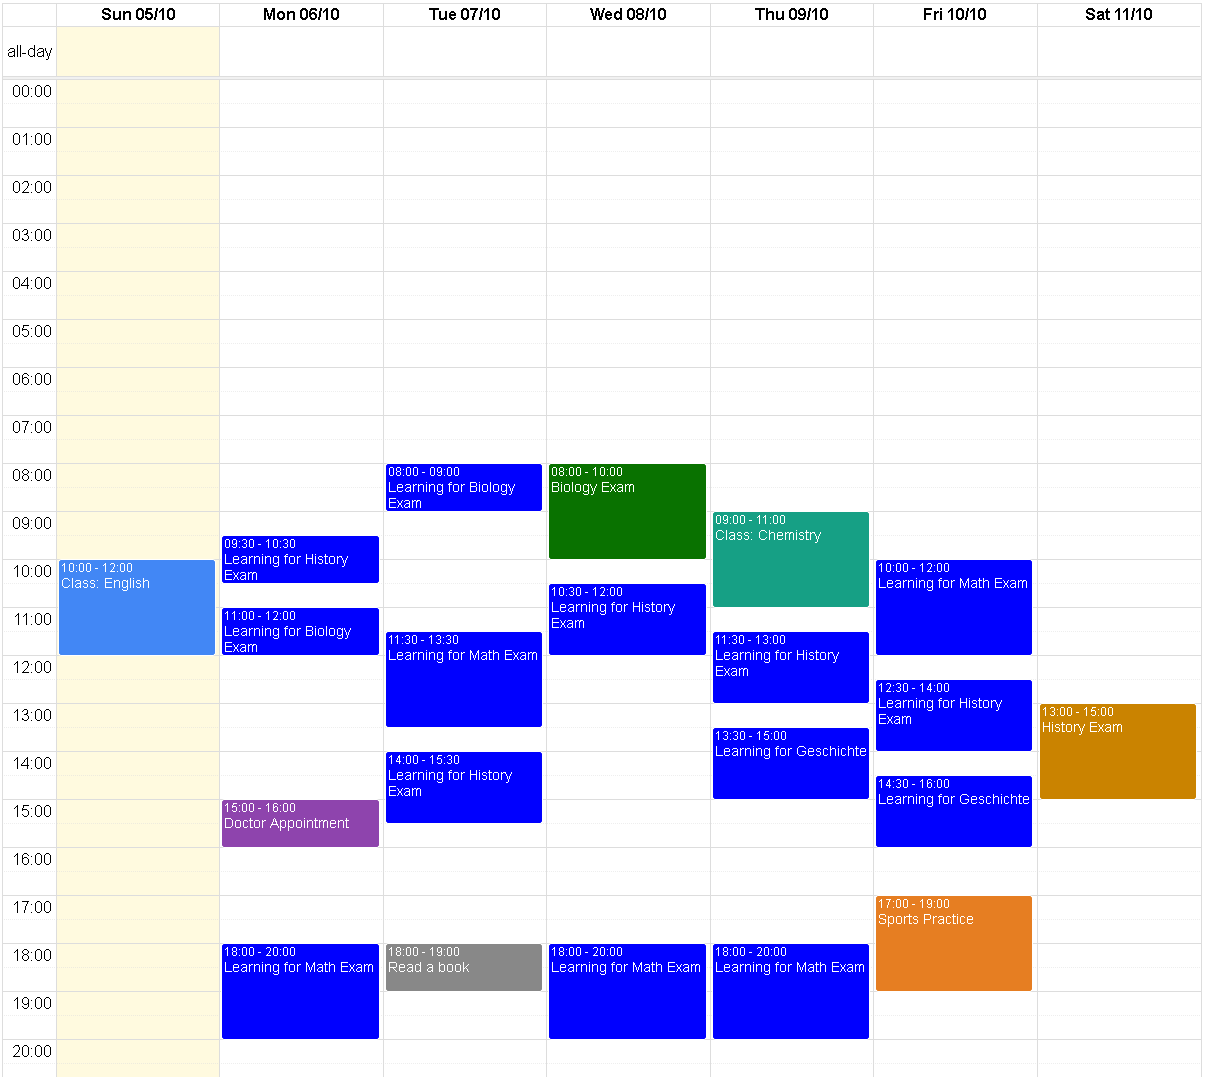
\includegraphics[width=\linewidth]{img/agenda.png}
    \caption{Beispiel einer Agenda, mit Lernblöcke von der LZA}
    \label{fig:placeholder}
\end{figure}
% ------------------------------ALGORITHMUS------------------------------
\subsection{Der Lernzeitalgorithmus}
Der Lernzeitalgorithmus (LZA) ist der Kern unserer Web-App. Er automatisiert die Planung der notwendigen Lernzeiten für die anstehenden Prüfungen eines Nutzers.

\subsubsection{Eingabeparameter und Planungsziel}

Der Lernzeitalgorithmus (LZA) verwendet globale Benutzereinstellungen sowie prüfungsspezifische Prioritätseinstellungen als Eingabeparameter, um eine optimale Lernplanung zu gewährleisten.

Das zentrale Planungsziel des LZA ist es, die definierten totale Lernstunden für jede Prüfung innerhalb des gültigen Lernfensters zu erreichen, während das tägliche Maximum und alle bestehenden Kalenderkonflikte des Nutzers strikt eingehalten werden.

\myparagraph{Globale Parameter}
Diese Einstellungen gelten für den gesamten Planungszeitraum:
\begin{itemize}
    \item \textbf{Lernen am Samstag}\\
    Definiert, ob der Algorithmus Lernblöcke an Samstagen planen darf.
    \item \textbf{Lernen am Sonntag}\\
    Definiert, ob der Algorithmus Lernblöcke an Sonntagen planen darf.
    \item \textbf{Bevorzugte Lernzeit}\\
    Die bevorzugte Uhrzeit am Tag, zu der die Platzierung von Lernblöcken primär angestrebt wird.
\end{itemize}

\myparagraph{Prüfungsspezifische Parameter (Pro Prioritätstufe)}
Diese Werte werden basierend auf der Priorität jeder Prüfung zugewiesen:
\begin{itemize}
    \item \textbf{Lernfenster}\\
    Die Anzahl der Tage rückwirkend ab dem Prüfungstermin, innerhalb derer Lernblöcke platziert werden sollen.
    \item \textbf{Tägliches Maximum}\\
    Die maximale Stundenzahl, die pro Tag für Prüfungen dieser Priorität geplant werden darf.
    \item \textbf{Total Lernstunden}\\
    Die gesamte Anzahl an Lernstunden, die für Prüfungen dieser Priorität absolviert werden muss.
\end{itemize}

\subsubsection{Ablauf und Planungsstrategie}
Der Algorithmus arbeitet iterativ und bearbeitet alle als Prüfung markierten Ereignisse in aufsteigender Reihenfolge ihrer Priorität. Eine niedrigere Prioritätsnummer kennzeichnet dabei eine höhere Wichtigkeit, um eine optimale Ressourcenverteilung zu gewährleisten.

\begin{enumerate}
    \item \textbf{Zyklische Neuberechnung der Anforderungen (Recycling)}:
    \begin{itemize}
        \item \textbf{Flexibilitätsbereinigung}: Alle vom System selbst geplanten, aber nicht gesperrten (gesperrt sind die Blöcke, die vom Nutzer bearbeitet worden sind) Lernblöcke für die aktuelle Prüfung werden gelöscht. Dies ermöglicht eine dynamische, optimale Neuplanung, falls sich die Rahmenbedingungen (z.B. neue Events, geänderte Prioritätseinstellungen) geändert haben.
        \item \textbf{Soll-Stunden-Ermittlung}: Die noch zu erbringende Lernzeit wird neu berechnet. Hierbei werden alle bereits absolvierten Stunden sowie Stunden, die durch manuelle oder vom Nutzer gesperrte Blöcke abgedeckt sind, von den Gesamtsollstunden abgezogen.
    \end{itemize}
    \item \textbf{Rückwärts-Iterative Planung}:
    \begin{itemize}
        \item Die Planungsstrategie ist eine Rückwärtsiteration: Sie beginnt beim Prüfungstermin und arbeitet sich tageweise bis zum aktuellen Datum vor. Dieses Vorgehen stellt sicher, dass die Lernblöcke mit höchster Dringlichkeit (die Tage, die am nächsten zur Prüfung liegen) zuerst belegt werden.
        \item An jedem Tag wird die maximale Lernzeit für diese spezifische Prüfung ermittelt. Diese ergibt sich aus der Differenz zwischen dem täglichen Maximum und den Stunden, die bereits an diesem Tag für die Prüfung geplant wurden. Dadurch wird das tägliche Zeitlimit zuverlässig eingehalten und eine Überlastung vermieden.
    \end{itemize}
    \item \textbf{Platzierung und strikte Konfliktvermeidung}:
    \begin{itemize}
        \item \textbf{Bevorzugter Slot}: Es wird primär versucht, einen Lernblock in der vom Nutzer festgelegten bevorzugten Lernzeit zu platzieren.
        \item \textbf{Konfliktprüfung}: Die Verfügbarkeit des Slots wird gegen alle Kalendereinträge des Nutzers für den aktuellen Tag geprüft. Dabei wird ein 30-minütiger Puffer vor und nach jedem bestehenden Ereignis (wie Sport oder Arzttermin) beachtet, um knappe Überlappungen und unnötigen Stress zu vermeiden.
        \item \textbf{Alternative Slots}: Falls die bevorzugte Zeit belegt ist, sucht ein dediziertes Modul den grössten verfügbaren, konfliktfreien Zeitabschnitt des Tages, um die Platzierung zu maximieren.
        \item \textbf{Echtzeit-Aktualisierung}: Nach der erfolgreichen Generierung und Speicherung eines Lernblocks wird dieser sofort zur Liste der aktuellen Kalenderereignisse hinzugefügt. Dieser Mechanismus ist entscheidend, um sicherzustellen, dass alle unmittelbar nachfolgenden Planungsversuche am selben Tag diesen neu erstellten Block als bereits belegt berücksichtigen und somit Überlappungen ausgeschlossen sind.
    \end{itemize}
    \item \textbf{Notfallplanung (Erweitertes Zeitfenster)}:
    \begin{itemize}
        \item Falls die Gesamtlernstunden nach der iterativen Planung im primären Lernfenster noch nicht erreicht wurden, aktiviert der Algorithmus eine Notfallsuche.
        \item Diese sucht nach verfügbaren Plätzen in einem erweiterten, sekundären Zeitfenster. Dieses Fenster erstreckt sich maximal bis zum 21. Tag vor der Prüfung.
        \item Die Regeln des täglichen Maximums und der Konfliktvermeidung bleiben auch in diesem Notfallmodus strikt erhalten.
    \end{itemize}
    \item \textbf{Ergebnisrückgabe und Zusammenfassung}:
    \begin{itemize}
        \item Nachdem alle Prüfungen bearbeitet wurden, gibt der Algorithmus eine detaillierte Zusammenfassung des Planungsvorgangs zurück.
        \item Diese Zusammenfassung informiert den Nutzer in einem Popup über die Gesamtzahl der hinzugefügten Lernblöcke und die Gesamtstunden, die erfolgreich geplant wurden.
        \item Zusätzlich wird für jede einzelne Prüfung der Planungsstatus (erfolgreich / nicht erfolgreich) und die geplante Stundenanzahl angezeigt.
    \end{itemize}
\end{enumerate}


% ------------------------------DAILY TIPS------------------------------
\subsection{Daily Tipps}
Ein relativ wichtiges Feature unserer App sind die Daily Tipps. Es sollte jeden Tag ein neuer Tipp an den Nutzer gezeigt werden auf der Startseite, entweder über die Kantonsschule oder allgemeine Lerntipps. Die einfachste Möglichkeit, dies zu implementieren, ist eine simple Modulo-Rechnung. 
\[
\text{Tipp des Tages} = (\text{Tag des Jahres}) \bmod (\text{Anzahl der Tipps})
\]

Somit wird an einem bestimmten Tag nur einen Tipp gezeigt und über das ganze Jahr sollten alle Tipps gezeigt werden (da wir sowieso weniger als 365 Tipps haben).


% ------------------------------NOTENORGANISATION------------------------------

\subsection{Notenorganisation}
In der Kantonsschule muss man immer wieder Prüfungen schreiben. Die Noten, die man erhält, sind dann wichtig für die Promotion in die nächste Stufe. Deswegen haben wir ein Feature, in dem man seine Noten pro Semester speichern kann. Jedes Semester hat schon die jeweiligen Fächer, die man dann in diesem Semester haben würde, geladen. Man kann natürlich immer noch Fächer löschen und hinzufügen. Man kann mit diesem Feature dann seine Durchschnitte pro Fach und Semester sehen. Ebenfalls kann man mit dem Notenrechner sehen, welche Note man in einem Fach brauchen würde, um einen bestimmten Schnitt in diesem Fach zu haben.

% ------------------------------LERNTIMER------------------------------
\subsection{Lerntimer}
Ein weiteres wichtiges Feature unserer App ist der Lerntimer. Dieser Timer basiert auf der Pomodoro-Technik, welche im Recherche Teil dieses Bericht erklärt wurde. Mit der Recherche, die wir führten, fanden wir es wichtig, ein solcher Lerntimer zu implementieren, da es eine sehr effektive Lerntechnik ist. Der Timer hat die Standard-Einstellungen von 25 Minuten Lernen und 5 Minuten Pause, welche man aber auch ändern kann, falls man das möchte.

% ------------------------------LERNTIPPS------------------------------
\subsection{Lerntipps}
Ein weiteres Feature unserer App sind die Lerntipps. Diese sind in verschiedene Kategorien aufgeteilt, wie zum Beispiel Zeitmanagement, Pausenmanagement, Stressmanagement und Lernmethoden. In jeder Kategorie gibt es verschiedene wissenschaftlich fundierte Tipps, welche wir aus unserer Recherche und den Interviews gesammelt haben. Diese Tipps sollen den Nutzer:innen helfen, ihr Lernverhalten zu verbessern und effektiver zu lernen.

% References
\clearpage
%\addcontentsline{toc}{chapter}{Bibliography}
%\nocite{*}
%\printbibliography
\clearpage
\addcontentsline{toc}{chapter}{Literaturverzeichnis} % Changed from Bibliography/Quellen
\nocite{*}
\printbibliography[title={Literaturverzeichnis}]


\end{document}
